\documentclass[tikz,border=1.35mm]{standalone}

\definecolor{fvmadaptedge}{HTML}{8A7E7E}
\usetikzlibrary{arrows.meta}

\definecolor{splitred}{HTML}{AF2525}

% Triangular face before and after isotropic face splitting.
% Coordinates are in millimeters; y=-1mm keeps the SVG-style origin at top left.
\begin{document}
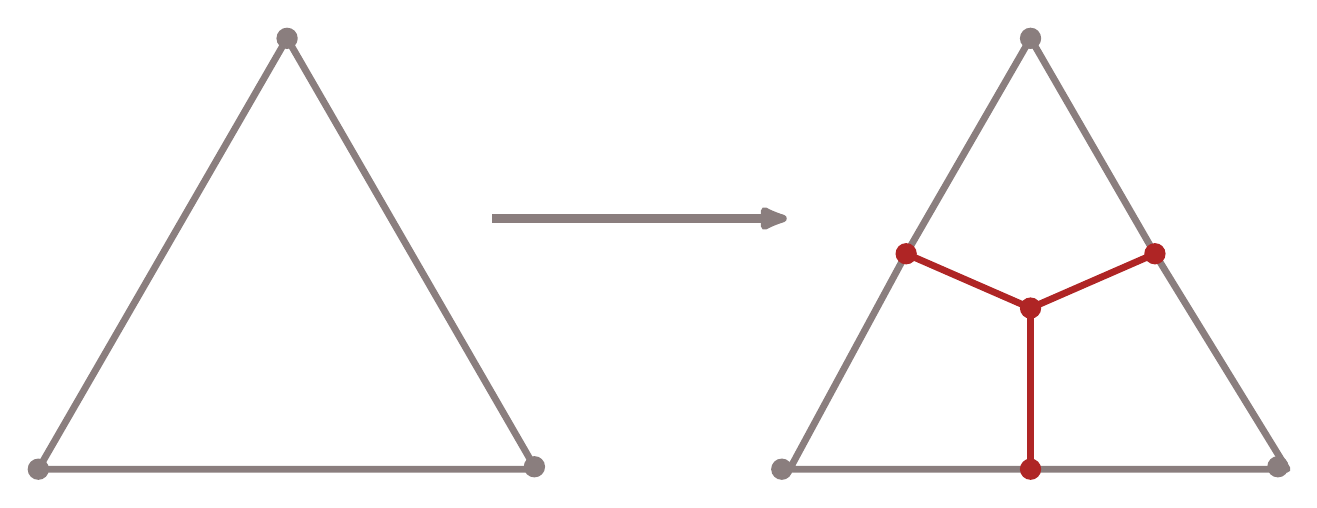
\begin{tikzpicture}[
  x=1mm,
  y=-1mm,
  line join=round,
  edge/.style={draw=fvmadaptedge,line width=0.865mm},
  splitline/.style={draw=splitred,line width=0.865mm},
  arrow/.style={draw=fvmadaptedge,line width=1.05mm,-{Latex[round,length=4.8mm,width=3.6mm]}}
]
  % Match the original artwork frame before the standalone border is applied.
  \useasboundingbox (0,0) rectangle (160.130,57.425);

  % Left panel: original unsplit triangle.
  \coordinate (leftA) at (1.353,56.073);
  \coordinate (rightA) at (64.538,56.073);
  \coordinate (topA) at (32.945,1.353);

  % Right panel: edge midpoints and face center created by the split.
  \coordinate (leftB) at (96.772,56.073);
  \coordinate (rightB) at (159.957,56.073);
  \coordinate (topB) at (127.364,1.353);
  \coordinate (leftMidB) at (111.568,28.713);
  \coordinate (rightMidB) at (143.161,28.713);
  \coordinate (bottomMidB) at (127.364,56.073);
  \coordinate (centerB) at (127.364,35.609);

  % Draw the old face and the split face topology.
  \draw[edge] (rightA) -- (leftA) -- (topA) -- cycle;
  \draw[edge] (leftMidB) -- (topB) -- (rightMidB) -- (rightB)
    -- (bottomMidB) -- (leftB) -- cycle;
  \draw[splitline] (centerB) -- (leftMidB);
  \draw[splitline] (centerB) -- (rightMidB);
  \draw[splitline] (centerB) -- (bottomMidB);

  % Transformation arrow between the before/after panels.
  \draw[arrow] (59.013,24.236) -- (96.402,24.236);

  % Original vertices are #8a7e7e.
  \fill[fvmadaptedge] (32.945,1.353) circle[radius=1.353mm];
  \fill[fvmadaptedge] (64.358,55.762) circle[radius=1.353mm];
  \fill[fvmadaptedge] (1.353,56.073) circle[radius=1.353mm];

  \fill[fvmadaptedge] (127.364,1.353) circle[radius=1.353mm];
  \fill[fvmadaptedge] (158.778,55.762) circle[radius=1.353mm];
  \fill[fvmadaptedge] (95.772,56.073) circle[radius=1.353mm];

  % Split-created edge and face nodes are red.
  \fill[splitred] (111.568,28.713) circle[radius=1.353mm];
  \fill[splitred] (143.161,28.713) circle[radius=1.353mm];
  \fill[splitred] (127.364,56.073) circle[radius=1.353mm];
  \fill[splitred] (127.364,35.609) circle[radius=1.353mm];
\end{tikzpicture}
\end{document}
